\section{Solving Recurrences}

\begin{frame}{The first example: Knuth Number(KN)}
We have the following example: 
\begin{align*}
    K_0 &= 1; \\
    K_{n+1} &= 1+ \min (2K_{\flr{n/2}}, 3K_{\flr{n/3}}).\\
\end{align*}
Prove or disproof that for $n \geq 0, K_n \geq n$. 

\begin{itemize}
    \item List small vals for $k$. 
    \item Proof by induction.
    \item Base case: $K=0$ satisfy the condition.
    \item Induction
\end{itemize}
    
\end{frame}

\begin{frame}{KN: Induction Step}
\begin{align*}
    K_0 &= 1; \\
    K_{n+1} &= 1+ \min (2K_{\flr{n/2}}, 3K_{\flr{n/3}}).\\
\end{align*}

\begin{itemize}
    \item Assume the inequality hold for all vals up to some 
    non negative vals $n$, 
    \item Goal: show that $K_{n+1} \geq n+1$. 
    \item Given $K_{n+1}=1+\min(2K_{\flr{n/2}}, 3K_{\flr{n/3}})$, 
    and $2K_{\flr{n/2}} \geq 2 \flr{n/2}, 3K_{\flr{n/3}}\geq 3\flr{n/3}$(by hypothesis) 
    \item But $2 \flr{n/2} $ can be as small as $n-1$, $3\flr{n/3}$ 
    can be as small as $n-2$, breaking the induction. 
    \item Or really? This case jumps fast.
\end{itemize}
    
\end{frame}

\begin{frame}{KN: The special case}
We can prove by contradiction: 
\begin{itemize}
    \item Assume we can find a value $m$ s.t. $K_m \leq m$
    \item finding $m$'s origin, say $m=n'+1$
    \item requires $K_{\flr{n'/2}}\leq \flr{n'/2}$, and $K_{\flr{n'/3}}\leq \flr{n'/3}$. 
    \item This implies $K_0 \leq 0$, but $K_0 = 1$, contradiction. 
\end{itemize}
    
\end{frame}

\begin{frame}{About Math. Induction}
\begin{columns}
\begin{column}{0.6\textwidth}
\begin{quote}
    In trying to devise a proof by mathematical induction, you may fail for two opposite reasons. You may fail because you try to prove too much: Your $P(n)$ is too heavy a burden. Yet you may also fail because you try to prove too little: Your $P(n)$ is too weak a support.
    
    In general, you have to balance the statement of your theorem so that the support is just enough for the burden."
\end{quote}
\end{column}

\begin{column}{0.4\textwidth}
\begin{figure}
    \centering
    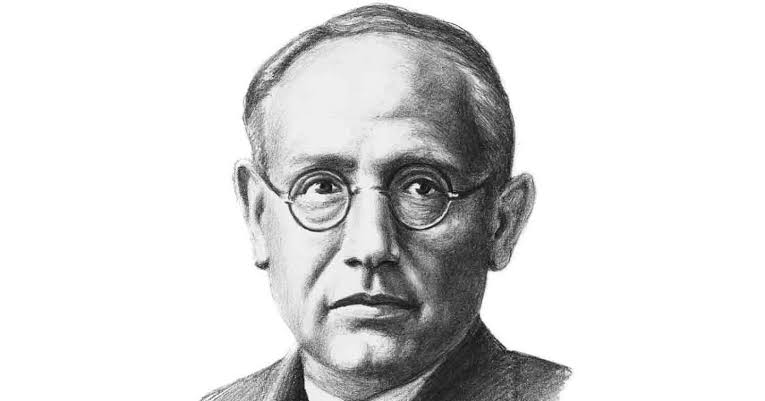
\includegraphics[width=\textwidth]{fig/ch3/gpolya.jpeg}
    \caption{G. Polya}
    \label{fig:induction}
\end{figure}
\end{column}

\end{columns}
    
\end{frame}

\begin{frame}{Jospher's Problem Generlized(JPG)}

Idea: Whenever a person is passed over, give it a \underline{new
number}. 

Demonstrate: \pause 
$$
\begin{array}{rrrrrrrrrr}1&2&3&4&5&6&7&8&9&10\\11&12&&13&14&&15&16&&17\\18&&&19&20&&&21&&22\\&&&23&24&&&&&25\\&&&26&&&&&&27\\&&&28&&&&&\\&&&29&&&&\\&&&30&&&&&\end{array}
$$
    
\end{frame}

\begin{frame}{JPG: Findings}
$$
\begin{array}{llllllllll}1&2&3^1&4&5&6^2&7&8&9^3&10\\11&12^4&&13&14&&15^5&16&&17\\18^6&&&19&20&&&21^7&&22\\&&&23&24^8&&&&&25\\&&&26&&&&&&27^9\\&&&28&&&&&\\&&&29&&&&\\&&&30^{10}&&&&&\end{array}
$$

\only<1-2>{
    What will the id become? 
    \begin{itemize}
        \item 1, 2 become \visible<2->{$n+1, n+2$};
        \item 3 executed; 
        \item 4, 5 become \visible<2->{$n+3, n+4$};
        \item 6 is executed;
        \item $3k+1, 3k+2$ will become \visible<2->{$n+2k+1, n+2k+2$};
        \item $3k+3$ is executed. 
    \end{itemize}
}

\only<3>{
\begin{itemize}
    \item Counting is consistent, no jumping over someone. 
    \item The $k$-th person eliminated ends up with number $3k$.
    \item To find the survivor = figure out the original number $3N$.
\end{itemize}
}

\only<4>{
    \begin{itemize}
        \item What is $3N$ originally? 
        \item $N(N>n)$ has a form of $N = n+2k+1$ or $N=n+2k +2$, in a single round. 
        \item for two $k$s, getting $k_1 = (N-1-n)/2, k_2=(N-2-n)/2$. 
        \item $=\flr{(N-n-1)/2}$. 
    \end{itemize}
}

\only<5>{
    An algorithm for this: 
    \begin{itemize}
        \item Let $N \leftarrow 3n$;
        \item while $N>n$, let $N\leftarrow \flr{(N-n-1)/2}+N-n$;
        \item Answer$\leftarrow N$.
    \end{itemize}
}

\only<6> {
    Simplifying this algorithm: like treating arithmetic series.
    \begin{itemize}
        \item Assign the numbers from largest to smallest
        \item yielding $\cil{3/2D}$. 
    \end{itemize}
}

\only<7> {
    Generalized: $D=\cil{q/(q-1)D}$ for general $q$s, i.e. $q$-kill one. 
}
    
\end{frame}

